\documentclass{beamer}

\usepackage[utf8]{inputenc}
\usepackage[brazil]{babel}
\usepackage{graphicx}

\usetheme{Madrid}

\title{Robótica na Educação Ambiental}
\subtitle{Cidadania Digital e Climática}
\author{Jefferson Bezerra dos Santos}
\date{}

\begin{document}

% Slide título
\frame{\titlepage}

% Introdução
\begin{frame}{Introdução}

\begin{columns}

\column{0.55\textwidth}

A crise ambiental e climática exige novas formas de educação.

A robótica educacional permite:

\begin{itemize}
\item integrar tecnologia e sustentabilidade
\item desenvolver pensamento científico
\item investigar problemas ambientais
\item criar soluções tecnológicas
\end{itemize}

\column{0.45\textwidth}

\centering

% Exemplo se quiser usar depois
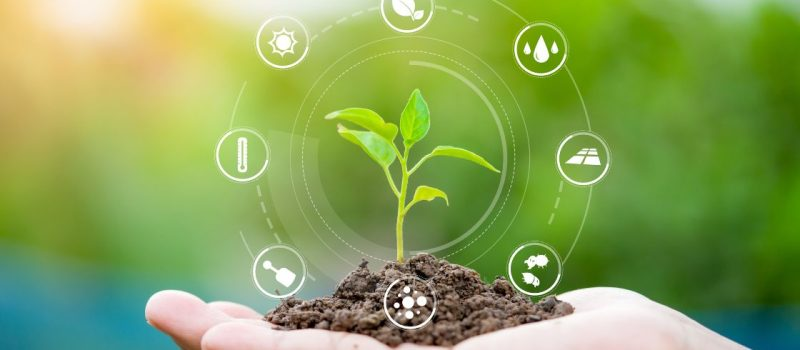
\includegraphics[width=\linewidth]{tecnologiaMeioAmbiente.jpg}

\end{columns}

\end{frame}

% Robótica educacional
\begin{frame}{Robótica Educacional}

\begin{columns}

\column{0.55\textwidth}

A robótica educacional utiliza tecnologias programáveis no ensino.

Ferramentas utilizadas:

\begin{itemize}
\item Arduino
\item sensores ambientais
\item microcontroladores
\item programação
\end{itemize}

Estimula criatividade, lógica e resolução de problemas.

\column{0.45\textwidth}

\centering

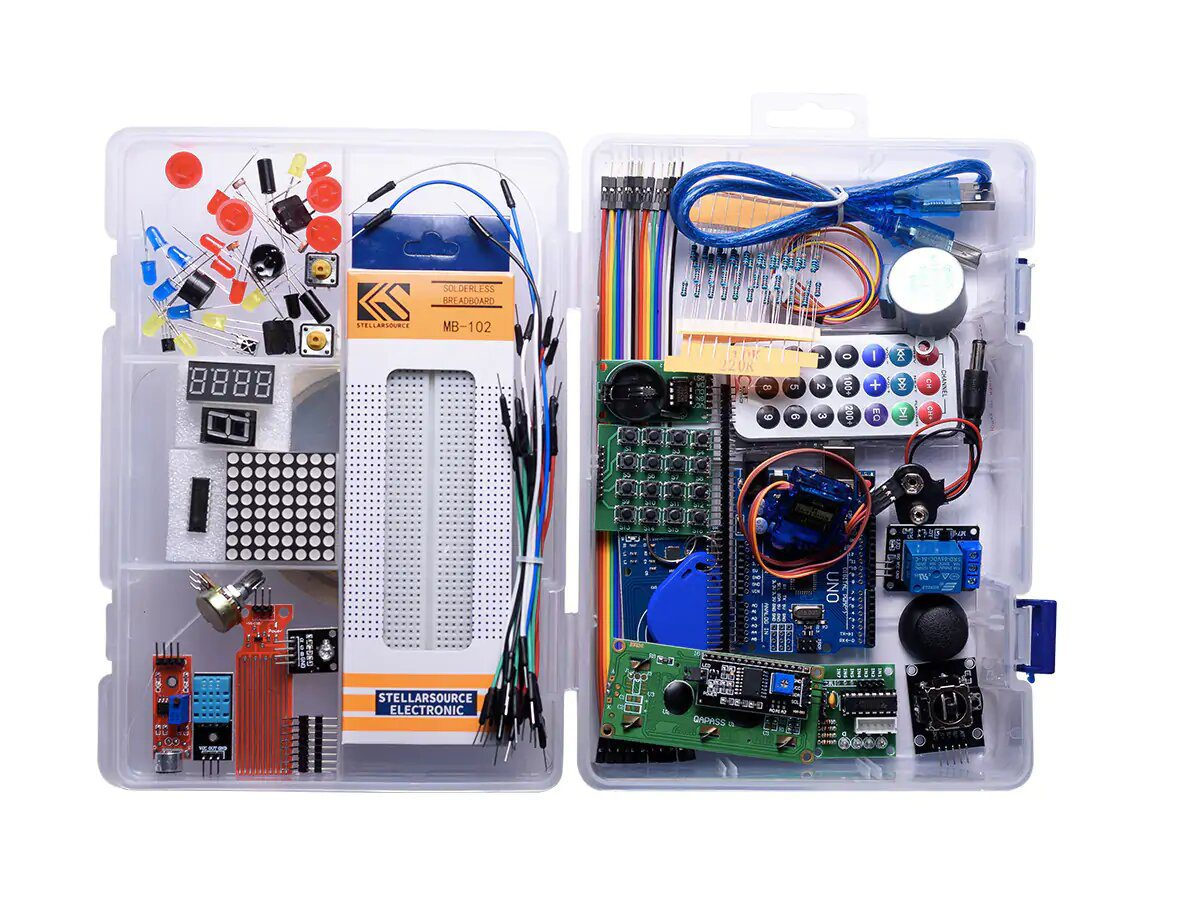
\includegraphics[width=\linewidth]{kitarduino.jpg}

\end{columns}

\end{frame}

% Educação ambiental
\begin{frame}{Educação Ambiental}

\begin{columns}

\column{0.55\textwidth}

A educação ambiental busca formar cidadãos capazes de:

\begin{itemize}
\item compreender problemas ambientais
\item desenvolver consciência ecológica
\item participar da preservação do planeta
\end{itemize}

Temas importantes:

\begin{itemize}
\item mudanças climáticas
\item poluição da água
\item sustentabilidade
\end{itemize}

\column{0.45\textwidth}

\centering
\fbox{\parbox[c][4cm][c]{5cm}{\centering Inserir imagem\\Educação Ambiental}}

\end{columns}

\end{frame}

% Cidadania digital
\begin{frame}{Cidadania Digital}

\begin{columns}

\column{0.55\textwidth}

Cidadania digital significa usar tecnologia de forma:

\begin{itemize}
\item responsável
\item ética
\item crítica
\item consciente
\end{itemize}

Aplicações:

\begin{itemize}
\item coleta de dados ambientais
\item análise de informações
\item compartilhamento científico
\end{itemize}

\column{0.45\textwidth}

\centering
\fbox{\parbox[c][4cm][c]{5cm}{\centering Inserir imagem\\Tecnologia e Dados}}

\end{columns}

\end{frame}

% Cidadania climática
\begin{frame}{Cidadania Climática}

\begin{columns}

\column{0.55\textwidth}

A cidadania climática envolve:

\begin{itemize}
\item compreender mudanças climáticas
\item desenvolver ações sustentáveis
\item utilizar tecnologia para monitoramento ambiental
\end{itemize}

Os estudantes tornam-se protagonistas na construção de soluções ambientais.

\column{0.45\textwidth}

\centering
\fbox{\parbox[c][4cm][c]{5cm}{\centering Inserir imagem\\Mudanças Climáticas}}

\end{columns}

\end{frame}

% Projetos
\begin{frame}{Projetos com Robótica}

Exemplos de projetos escolares:

\begin{itemize}
\item monitoramento da qualidade da água
\item estação meteorológica escolar
\item sensores ambientais
\item robôs para coleta seletiva
\end{itemize}

\bigskip

\centering
\fbox{\parbox[c][4cm][c]{8cm}{\centering Inserir imagem\\Projeto desenvolvido pelos alunos}}

\end{frame}

% Projeto Arduino
\begin{frame}{Exemplo de Projeto}

Projeto: Monitoramento da Qualidade da Água

Sensores utilizados:

\begin{itemize}
\item turbidez
\item temperatura
\item TDS
\item sensor de cor da água
\end{itemize}

\bigskip

\centering
\fbox{\parbox[c][4cm][c]{8cm}{\centering Inserir imagem\\Arduino + Sensores}}

\end{frame}

% Metodologias
\begin{frame}{Aprendizagem Ativa}

A robótica favorece metodologias como:

\begin{itemize}
\item aprendizagem baseada em projetos
\item cultura maker
\item investigação científica
\item trabalho colaborativo
\end{itemize}

\bigskip

\centering
\fbox{\parbox[c][4cm][c]{8cm}{\centering Inserir imagem\\Alunos construindo projetos}}

\end{frame}

% Conclusão
\begin{frame}{Conclusão}

A robótica educacional aplicada à educação ambiental permite:

\begin{itemize}
\item aprendizagem significativa
\item desenvolvimento da cidadania digital
\item compreensão das mudanças climáticas
\end{itemize}

\bigskip

\centering
\fbox{\parbox[c][4cm][c]{8cm}{\centering Inserir imagem\\Tecnologia e Sustentabilidade}}

\end{frame}

\begin{frame}
\centering
\Huge Obrigado!
\end{frame}

\end{document}
